\documentclass[]{article}

\usepackage[utf8]{inputenc}
\usepackage{amsmath}
\usepackage{amssymb}
\usepackage{amsthm}
\usepackage{amsfonts}
\usepackage{graphicx}
\usepackage{capt-of}
\usepackage{listings}
\usepackage{siunitx}
\usepackage[section]{placeins}
\usepackage{float}



% Oppgavenummerering %
\renewcommand\thesection{Problem \arabic{section}}
\renewcommand\thesubsection{\alph{subsection})}
\renewcommand\thesubsubsection{\alph{subsection}.\arabic{subsubsection})}

% Bevis
\newcommand\TombStone{\rule{.5em}{.5em}}
\renewcommand\qedsymbol{\TombStone}
\renewcommand{\proofname}{Bevis.} % Norske bevis

\title{TTK4215 - Assignment 7}
\author{Sigurd Totland | MTTK}

\begin{document}
\maketitle

\section{I\&S 4.13 d, e}
\setcounter{subsection}{3}
\subsection{}
\subsubsection{Adaptive law derivation}
We write the system with the common bilinear parametrization
\begin{equation}\begin{aligned}
y &= \frac{1}{k}(u - ms^2y - \beta sy) \\
&= \rho^* \left(
-\begin{bmatrix}
\beta & m \\
\end{bmatrix}
\begin{bmatrix}
sy\\
s^2y\\
\end{bmatrix}
+ u \right).
\end{aligned}\end{equation}
Because we have derivatives, We need to filter this with at least a second-order filter to make it realizable. We choose $W(s)L(s) = \frac{1}{\Lambda(s)}$ as our filter, where $\Lambda(s)$ is a second order Hurwitz polynomial in $s$. With that, we can write
\begin{equation}\begin{aligned}
z = \frac{y}{\Lambda}
&= W(s)L(s) \rho^* (\theta^{*\top}\phi + z_1) \\
 &= \frac{1}{\Lambda(s)} \rho^*
\left(
\begin{bmatrix}
\beta & m \\
\end{bmatrix}
\begin{bmatrix}
s\\
s^2\\
\end{bmatrix}
(-y)
+ u \right),
\end{aligned}\end{equation}
where $\theta^{* \top} = \begin{bmatrix} \beta & m \end{bmatrix}$,
$\rho^* = \frac{1}{k}$,
$\phi = \begin{bmatrix} s & s^2 \end{bmatrix}^\top (-y)$ and $z_1 = u$.
This let's us use an adaptive law from table 4.4 in I\&S, namely
\begin{equation}\begin{aligned}
\dot \theta = \Gamma \epsilon \phi \text{sgn}(\rho^*) = \Gamma \epsilon \phi
\end{aligned}\end{equation}
since we know a priori that $\text{sgn}(\rho^*) = 1$, as well as
\begin{equation}\begin{aligned}
\label{eq:adap_rho}
\dot \rho = \gamma \epsilon \xi.
\end{aligned}\end{equation}
We here define the estimation error to be
\begin{equation}\begin{aligned}
\epsilon = z - \hat z.
\end{aligned}\end{equation}
Note that we have let the normalization term $n_s^2 = 0$. Furthermore, we have
\begin{equation}\begin{aligned}
\xi = \theta^\top \phi + z_1.
\end{aligned}\end{equation}
Finally, $\hat z$ is defined as
\begin{equation}\begin{aligned}
\label{eq:z_hat}
\hat z = W(s)L(s)\rho(\theta^\top \phi + z_1) = \frac{1}{\Lambda}\rho (\theta^\top \phi + u)
\end{aligned}\end{equation}

\subsubsection{Simulation with constant mass}
When simulating this, we filter $\phi$ and $\rho$ individually since
\begin{equation}\begin{aligned}
\hat z = \frac{1}{\Lambda}\rho (\theta^\top \phi + u)
= \rho(\frac{1}{\Lambda}\theta^\top \phi + \frac{1}{\Lambda} u).
\end{aligned}\end{equation}
From this, we also note that
\begin{equation}\begin{aligned}
\label{eq:z_hat_xi}
\hat z = \rho \frac{1}{\Lambda}\xi,
\end{aligned}\end{equation}
i.e. $\xi$ filtered with our stable filter and scaled by $\rho$. This let's us calculate the filtered $\xi$ and then use it for both \eqref{eq:adap_rho} and \eqref{eq:z_hat_xi}. The main simulation loop that achieves this is shown in listing 1.

\begin{lstlisting}[basicstyle=\tiny, caption={Main simulation loop}]
% Main simulation loop
for n = 1:N-1
    % Generate input
    t(n+1) = n*h;
    u = 10*sin(2*t(n)) + 10*cos(3.6*t(n)) + 20*cos(1*t(n));
    U(n) = u;

    % Changing mass after t = 20s
    if(varying_mass && t(n) > 20)
        m = 20*(2-exp(-0.01*(t(n) - 20)));
        A = [0, 1; -k/m, -beta/m];
        B = [0; 1/m];
    end

    % Save actual model parameters at timestep for comparison later
    theta_star(:, n+1) = [beta, m];
    rho_star(:, n+1) = k;

    % Simulate actual system
    x_dot = A*x(:, n) + B*U(n);
    x(:, n+1) = x(:, n) + h*x_dot;
    y = x(1, n);

    % Calculate z
    x_z_n = x_z + (A_f*x_z + B_f*y)*h; % Euler integration
    z = C_f_1*x_z; % Fetch output

    % Calculate phi
    x_phi_n = x_phi + (A_f*x_phi + B_f*(-y))*h; % Euler integration
    phi_filt = [C_f_2*x_phi + D_f_2*(-y); C_f_3*x_phi + D_f_3*(-y);]; % Fetch output

    % Calculate z_1 = u_filt
    x_u_filt_n = x_u_filt + (A_f*x_u_filt + B_f*u)*h; % Euler integration
    u_filt = C_f_1*x_u_filt; % Fetch output


    % Calculate z_hat
    xi_filt = theta(:, n)'*phi_filt + u_filt;
    z_hat = rho(:, n)*xi_filt;

    % Estimation error
    epsilon = z - z_hat;

    % Propagate parameter estimates using Euler intagration
    theta_dot = Gamma*epsilon*phi_filt;
    theta(:, n+1) = theta(:, n) + theta_dot*h;

    rho_dot = gamma_k * epsilon * xi_filt;
    rho(:, n+1) = rho(:, n) + rho_dot * h;

    % Set variables for next iteration
    x_phi = x_phi_n;
    x_z = x_z_n;
    x_u_filt = x_u_filt_n;
end
\end{lstlisting}
The results are shown in figure \ref{fig:const_mass}.
\begin{figure}[H]
\centering
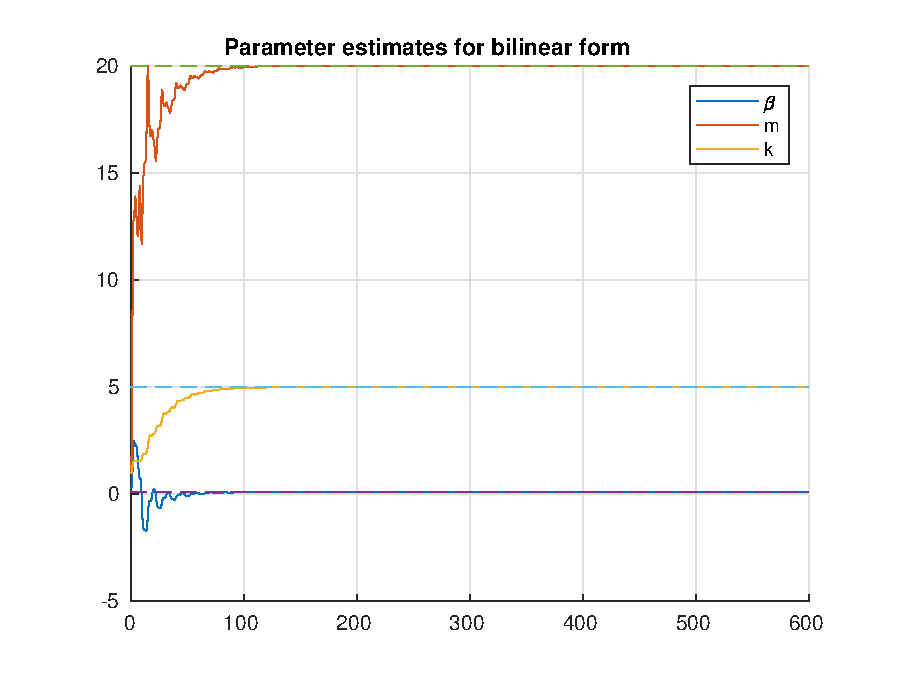
\includegraphics[width=0.75\textwidth]{const_mass.eps}
\caption{Parameter estimation using bilinear form}
\label{fig:const_mass}
\end{figure}

\subsection{Varying mass}
Letting the mass equal
\begin{equation}\begin{aligned}
m = 20(2 - e^{-0.01(t-20)})
\end{aligned}\end{equation}
for $t \geq 20$, we get the results shown in figure \ref{fig:varying_mass}.
\begin{figure}[H]
\centering
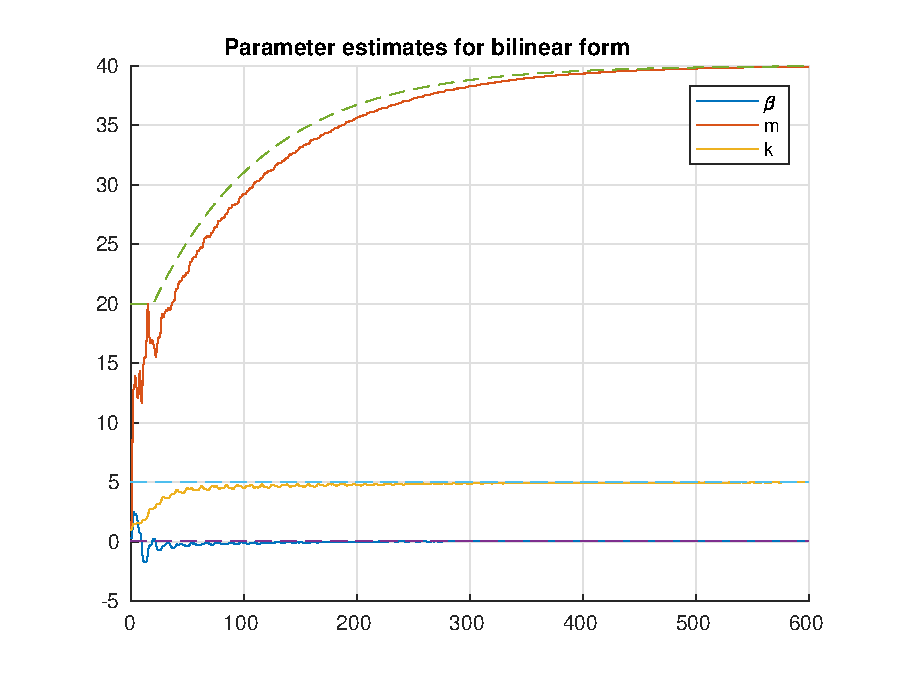
\includegraphics[width=0.75\textwidth]{varying_mass.eps}
\caption{Bilinear form parameter estimation with varying mass}
\label{fig:varying_mass}
\end{figure}

\end{document}

